\documentclass{beamer}
\usepackage{graphicx,tabularx}
\usepackage{amsmath}
\usepackage{multicol}

\graphicspath{ {./source/} }
\usepackage[utf8]{inputenc}

\title{Comparison of network complexity measures}
\author{Yipei Zhao}
\institute{Aston University}
\date{\today}

\begin{document}
    \frame{\titlepage}
    \begin{frame}{Network Science}
        \centering
        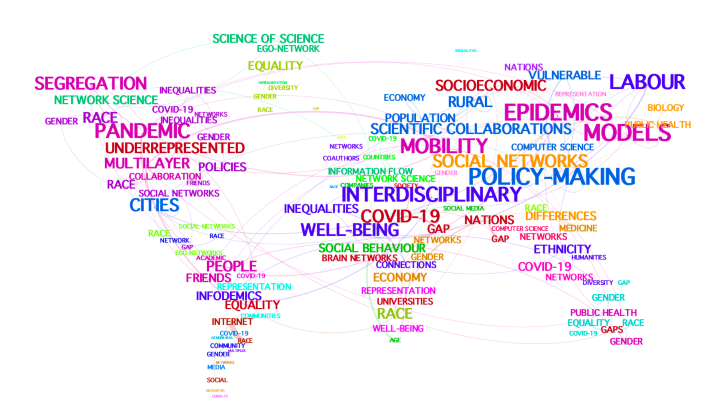
\includegraphics[width=\textwidth]{v1.png}
        {\url https://appliednetsci.springeropen.com/networked-inequality-\-studies-on-diversity-and-marginalization}
    \end{frame}

    \begin{frame}{Complexity measures}
        \begin{itemize}
            \item Different subgraph measures
            \begin{itemize}
                \item $C_{1e,st}$; counting the number of different subgraphs with different number of spanning trees after deleting one edge.
                \item $C_{1e,spec}$; counting the number of different subgraphs with different spectrums after deleting one edge.
                \item $C_{2e,spec}$; counting the number of different subgraphs with different spectrums after deleting two edges.
            \end{itemize}
            \item Product measures
            \begin{itemize}
                \item $MA_g$; product of redundancy and mutual information.
                \item $MA_{RI}$; product of redundancy and mutual information using a different normalisation method than $MA_g$.
                \item $Cr$; largest eigenvalue of adjacency matrix.
                \item $Ce$; efficiency of the graph.
            \end{itemize}
            \item Entropy measure
            \begin{itemize}
                \item $OdC$; calculating the entropy of node-node link correlation matrix.
            \end{itemize}
        \end{itemize}
    \end{frame}


    \begin{frame}{$MA_{RI}$}
        A product measure that is based on the idea of $MA_g$.
        \begin{itemize}
            \item Redundancy of a graph: $R=\frac{1}{m}\sum_{i,j>i}ln(d_id_j)$
            \item Mutual information of a graph: $I=\frac{1}{m}\sum_{i,j>i}ln(\frac{2m}{d_id_j})$
            \item An alternative way to state the mutual information: $I=ln(2m)-R$
            \item Highest redundancy: $R_{clique} = 2ln(n-1)$
            \item Lowest redundancy: $R_{path} = 2(\frac{n-2}{n-1})ln(2)$
            \item Highest mutual information: $I_{path} = ln(n-1)-(\frac{n-3}{n-1})ln2$
            \item Lowest mutual information: $I_{clique}=ln(\frac{n}{n-1})$
        \end{itemize}
        We can define the complexity to be $C = (R - R_{path})(I-I_{clique})$.\\
        $MA_g=16(\frac{R-R_{path}}{R_{clique}-R_{path}})(1-\frac{R-R_{path}}{R_{clique}-R_{path}})(\frac{I-I_{clique}}{I_{path}-I_{clique}})(1-\frac{I-I_{clique}}{I_{path}-I_{clique}})$
    \end{frame}

    \begin{frame}{$MA_{RI}$ continue}
        To compare different complexity measures, they need to be normalised: $0<C<1$.\\
        The complexity measure can be rewritten as: $C=(R-R_{path})(ln(2m)-R-I_{clique})$.\\
        \vspace{5mm}
        \centering
        $C = -R^2+(ln(2m)-I_{clique}+R_{path})R+(-R_{path}ln(2m)+R_{path}I_{clique})$
    \\
        \vspace{5mm}
        $R_{max} = \frac{ln(2m)-I_{clique}+R_{path}}{2}$\\
        \vspace{5mm}
        $C_{max} = \frac{(ln(2m)-I_{clique}-R_{path})^2}{4}$\\
        \vspace{5mm}
        $MA_{RI} = \frac{4(R-R_{path})(I-I_{clique})}{(ln(2m)-I_{clique}-R_{path})^2}$
    \end{frame}

    \begin{frame}{Result}
        \begin{multicols}{3}
            \centering
            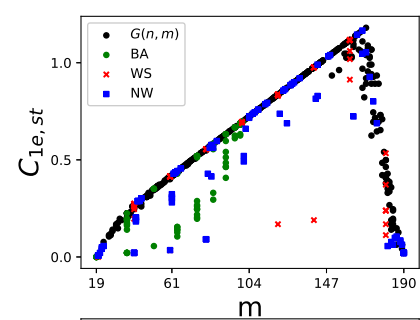
\includegraphics[width=0.3\textwidth,height=0.3\textheight,keepaspectratio]{1.png}
            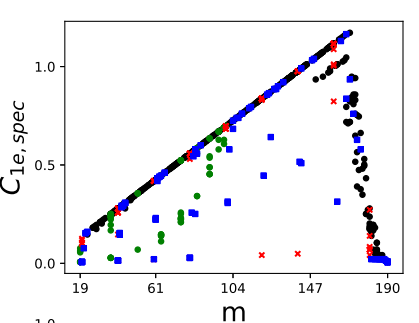
\includegraphics[width=0.3\textwidth,height=0.3\textheight,keepaspectratio]{2.png}
            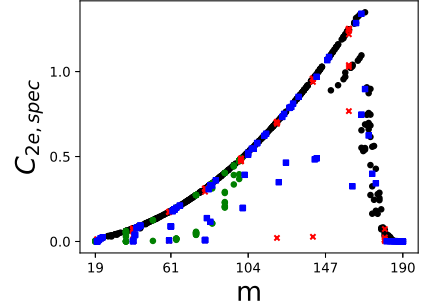
\includegraphics[width=0.3\textwidth,height=0.3\textheight,keepaspectratio]{3.png}
        \end{multicols}
        \begin{multicols}{3}
            \centering
            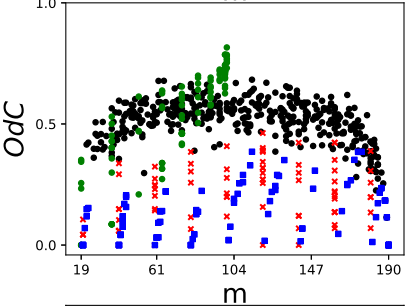
\includegraphics[width=0.3\textwidth,height=0.3\textheight,keepaspectratio]{4.png}
            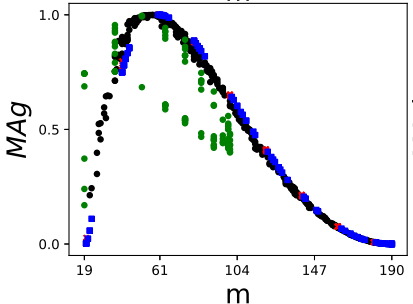
\includegraphics[width=0.3\textwidth,height=0.3\textheight,keepaspectratio]{5.png}
            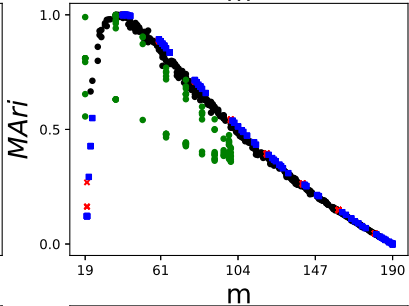
\includegraphics[width=0.3\textwidth,height=0.3\textheight,keepaspectratio]{6.png}
        \end{multicols}
        \begin{multicols}{2}
            \centering
            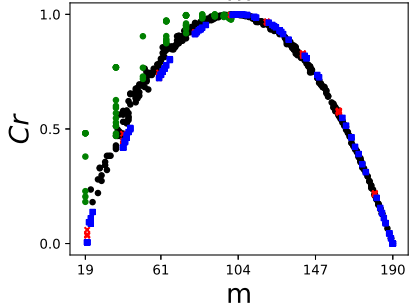
\includegraphics[width=0.5\textwidth,height=0.3\textheight,keepaspectratio]{7.png}
            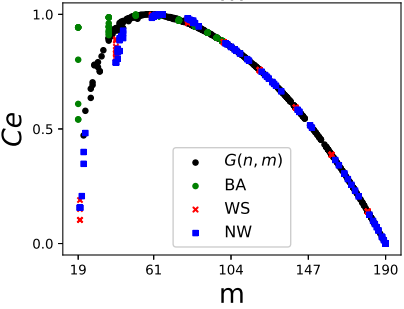
\includegraphics[width=0.5\textwidth,height=0.3\textheight,keepaspectratio]{8.png}
        \end{multicols}
    \end{frame}

    \begin{frame}{Result continue}
        \vspace{-5mm}
            \begin{figure}
                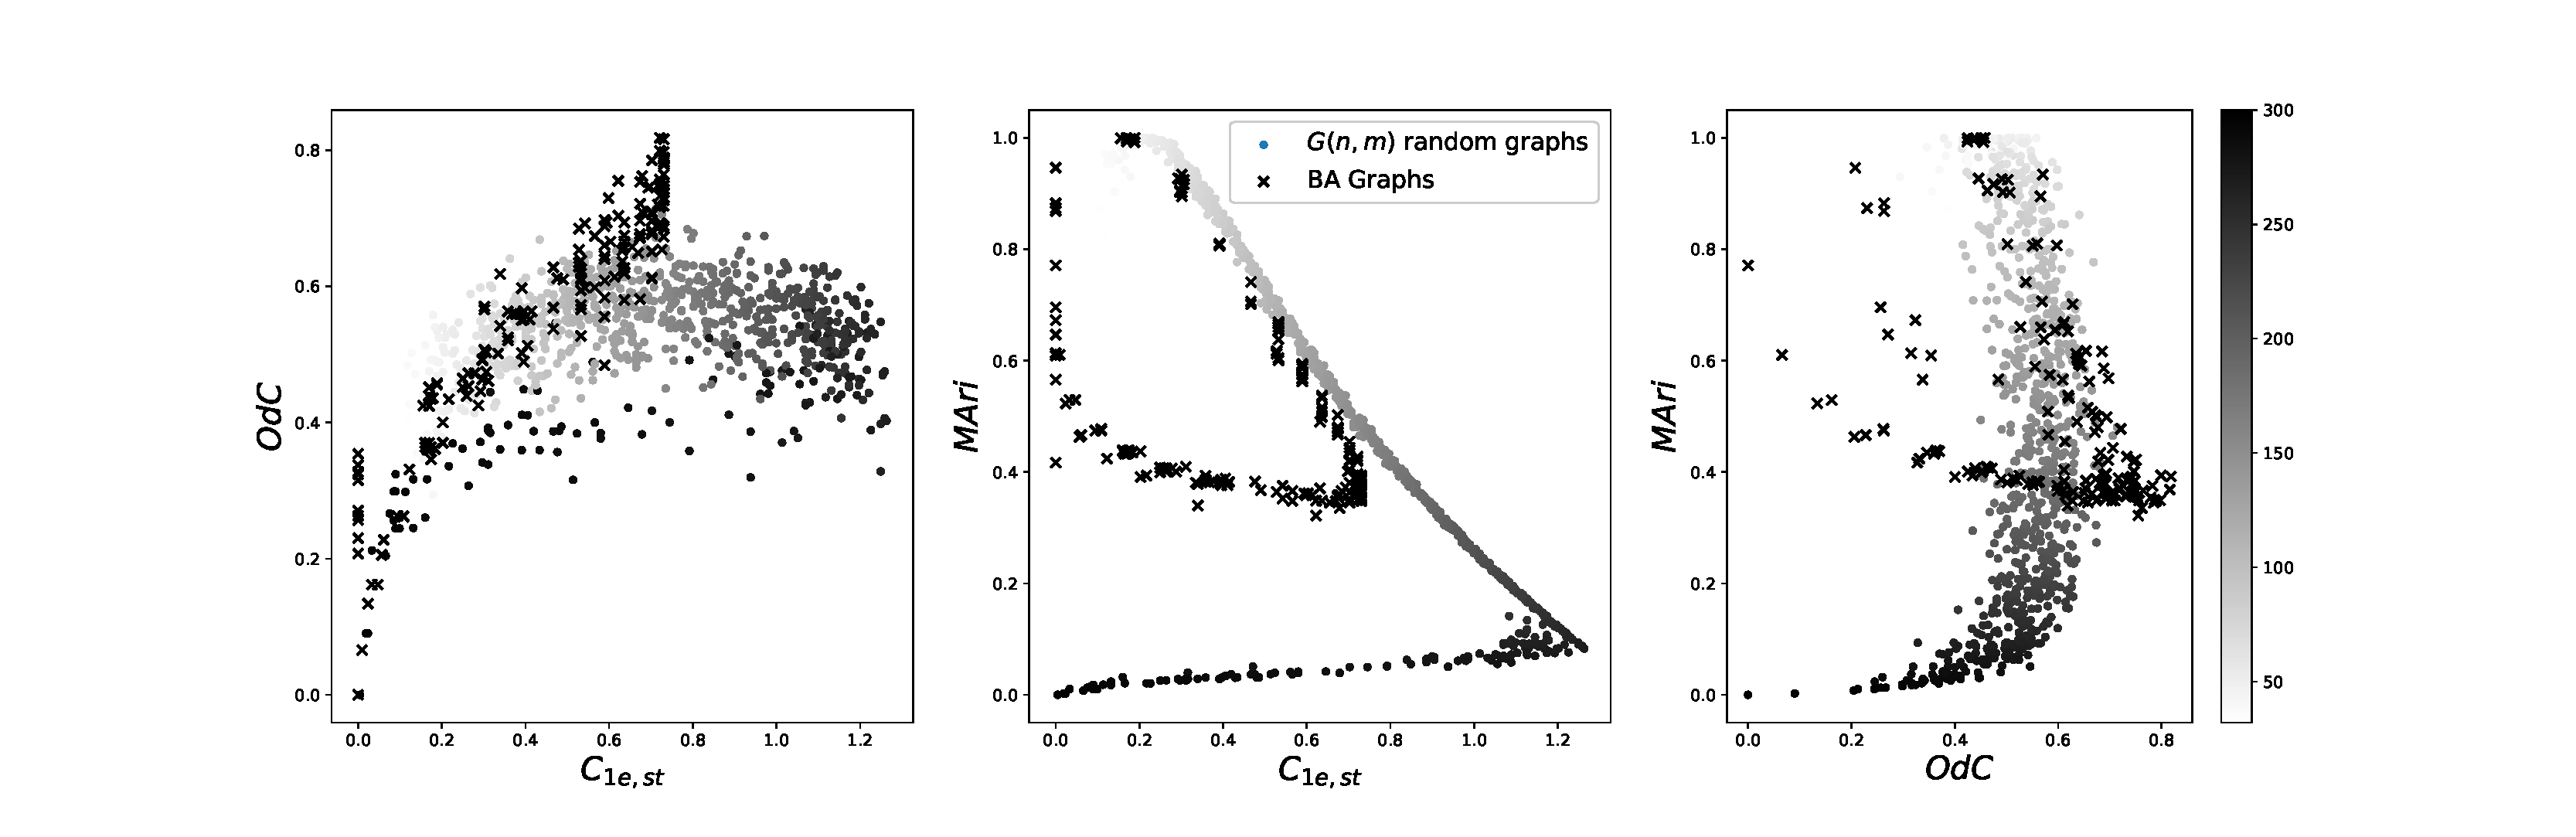
\includegraphics[width=\textwidth,height=0.5\textheight,keepaspectratio]{complexity_correlation.eps}
                \vspace{-10mm}
                \caption{Correlation between complexity measures, all graphs have 25 nodes and random number of edges. The darker the data point, the graph has more number of nodes.}
            \end{figure}
            \vspace{-15mm}
            \begin{figure}
                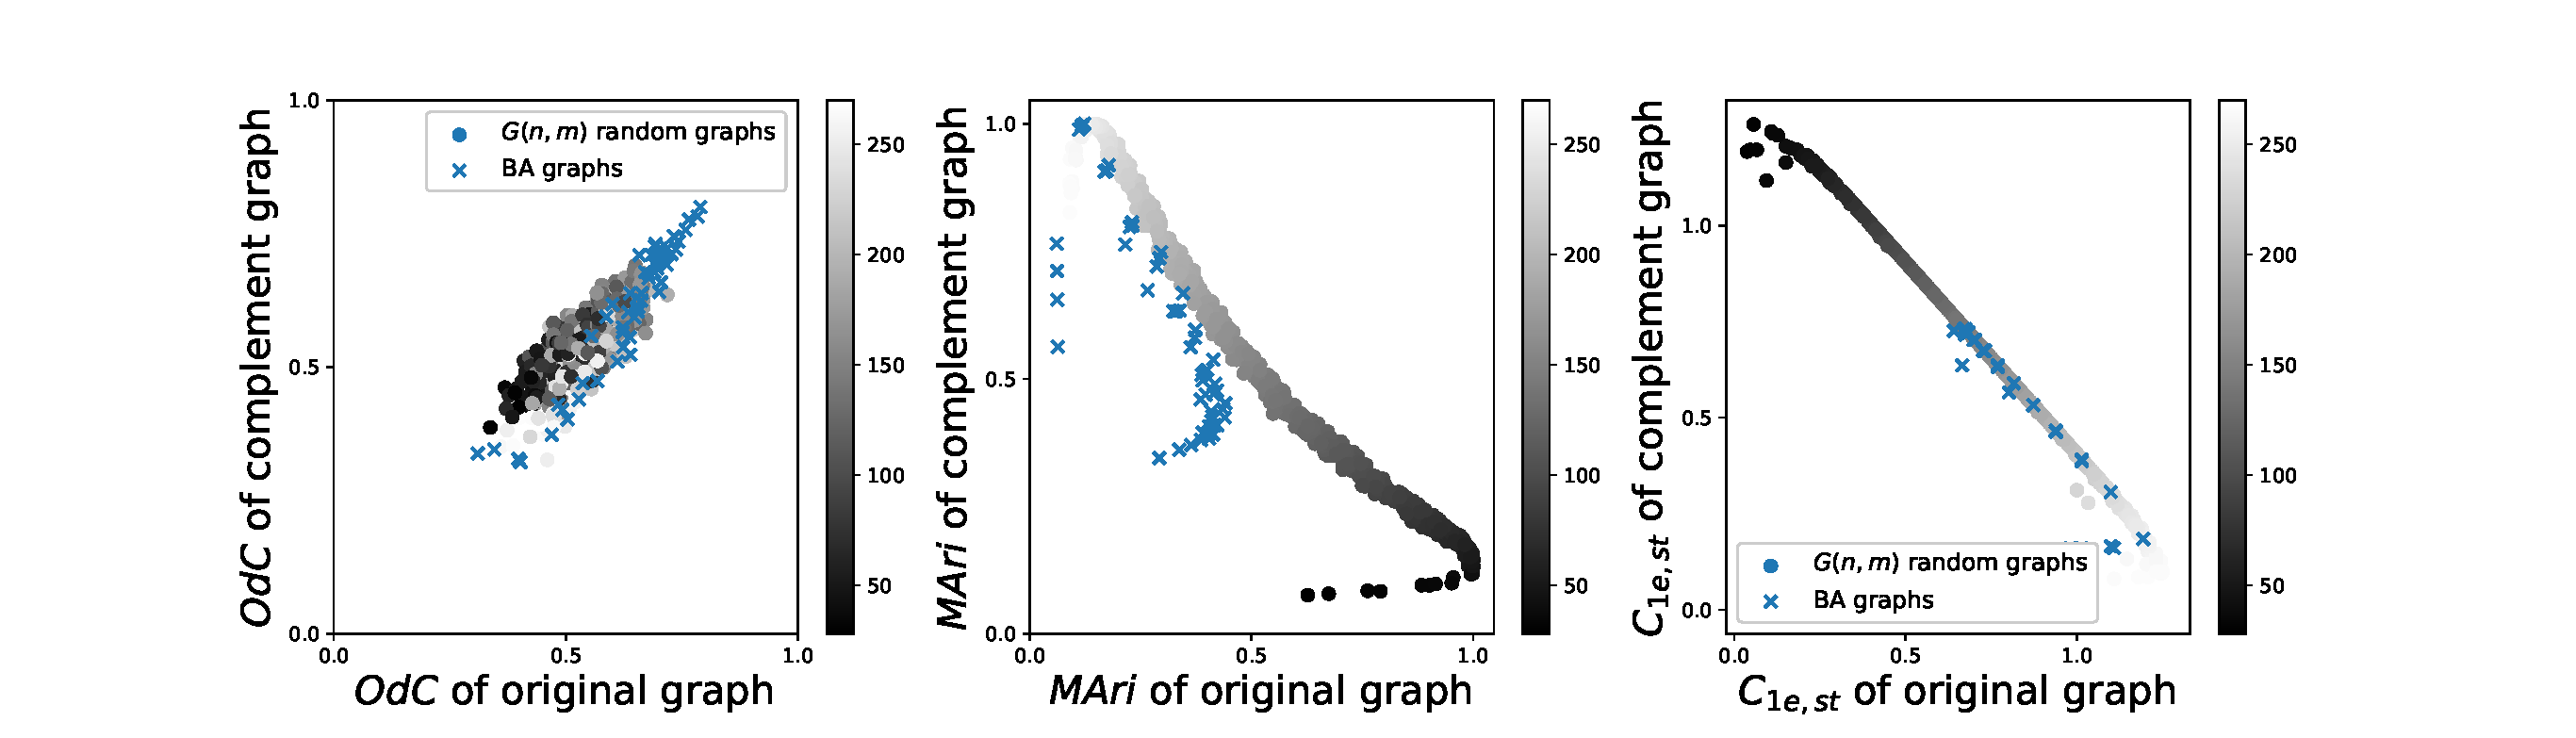
\includegraphics[width=\textwidth,height=0.5\textheight,keepaspectratio]{complement.eps}
                \caption{ Complexities of the original graphs and complement graphs with $n = 20$.}
            \end{figure}
    \end{frame}

    \begin{frame}{Result continue}
        
        \makebox[\textwidth][c]{
        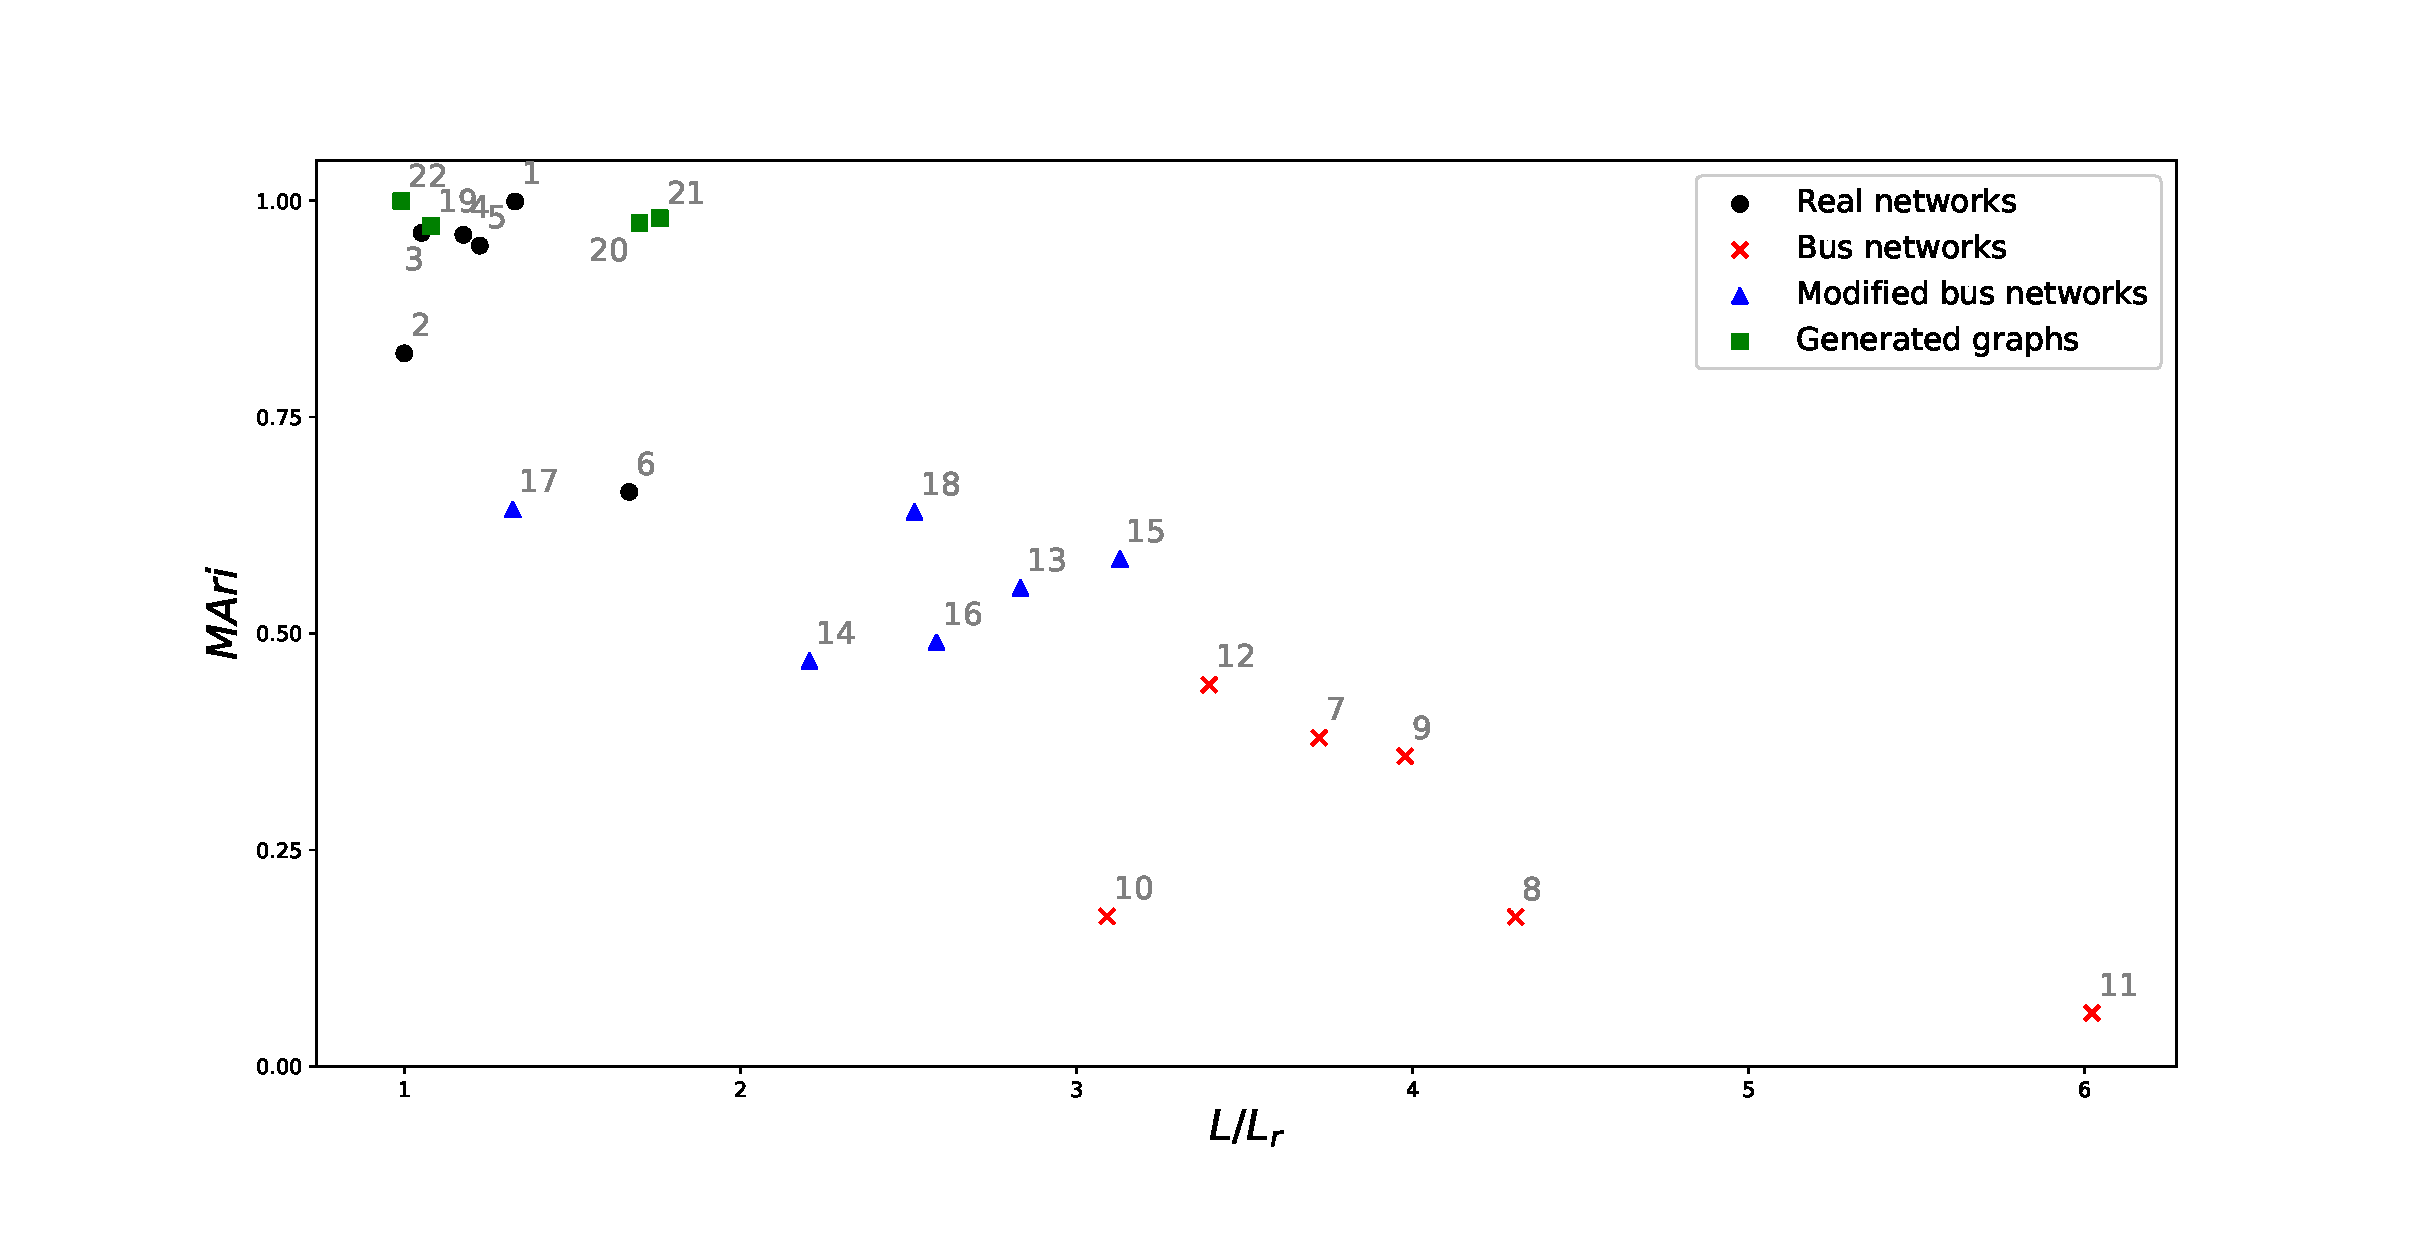
\includegraphics[width = 1.4\textwidth]{real_networks.eps}}
        \centering
        $MA_{RI}$ complexity of real networks, bus networks, modified bus networks and graphs generated by graph models.
    \end{frame}

    \begin{frame}{Conclusion}
        \begin{itemize}
            \item Compared different complexity measures
            \item Introduced $MA_{RI}$
            \item Compared complexity measures on different types of graph
            \item Investigated the uniqueness of transportation networks
            \item How to invent an optimal complexity measure?
            \item Do transportation networks require different complexity measures compare to other real networks?
            \item Should different type of networks use different measure?
        \end{itemize}
    \end{frame}

    \begin{frame}{Question time}
        \centering

        {\Huge Any question for me?}
    \end{frame}
\end{document}